\chapter{Profiling: Nsight, Occupancy, and Roofline}\label{ch:profiling}

\begin{center}\small\textit{You cannot optimise what you cannot measure --- profile first, hypothesise, then code.}\end{center}

\noindent\fbox{\parbox{\dimexpr\linewidth-2\fboxsep-2\fboxrule}{%
\textbf{From zero: measurement before magic.} We treat the GPU as a black box with counters. Profiling reveals whether time is spent computing, moving data, or waiting idle. We start with a mental model (time breakdown), then tools that fill it with numbers: Nsight Systems for the big picture, Nsight Compute for the kernel, and the roofline for the verdict.}}
\vspace{0.4em}

\section*{Learning Outcomes}
After this chapter you will be able to:
\begin{enumerate}[label=(L\arabic*)]
    \item run Nsight Systems and Compute to collect timelines and kernel metrics;
    \item interpret occupancy limits from registers, shared memory, and threadblock size;
    \item plot a roofline and classify kernels as memory- vs.\ compute-bound;
    \item use NVTX ranges to correlate source regions with GPU activity;
    \item design an iterative optimisation loop driven by profiler data.
\end{enumerate}

\section{The Profiling Mindset}
Optimisation without data is superstition. The first step is a \emph{time budget}: for an end-to-end run, what fraction is kernel compute, H2D/D2H copy, NCCL, and CPU overhead? If copies are 40\%, kernel tuning is premature --- hide copies with streams first.

Two complementary views: \emph{system} (Nsight Systems) shows CPU+GPU+NCCL on a shared timeline, answering ``what runs when and who waits?''; \emph{kernel} (Nsight Compute) shows one kernel's microarchitecture counters, answering ``why is this kernel slow?'' Use Systems first to find the bottleneck kernel, then Compute to fix it.

\begin{figure}[h]\centering
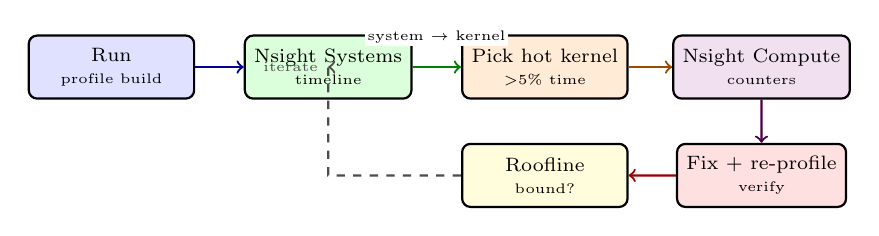
\begin{tikzpicture}[font=\scriptsize, scale=0.86,
  stage/.style={draw, thick, rounded corners=3pt, minimum width=2.1cm, minimum height=0.80cm, align=center}]
  \node[stage, fill=blue!12] (run) at (0,0) {Run\\{\tiny profile build}};
  \node[stage, fill=green!14] (sys) at (3.2,0) {Nsight Systems\\{\tiny timeline}};
  \node[stage, fill=orange!16] (k) at (6.4,0) {Pick hot kernel\\{\tiny >5\% time}};
  \node[stage, fill=violet!12] (comp) at (9.6,0) {Nsight Compute\\{\tiny counters}};
  \node[stage, fill=red!12] (fix) at (9.6,-1.6) {Fix + re-profile\\{\tiny verify}};
  \node[stage, fill=yellow!14] (roof) at (6.4,-1.6) {Roofline\\{\tiny bound?}};
  \draw[->, thick, blue!60!black] (run) -- (sys);
  \draw[->, thick, green!50!black] (sys) -- (k);
  \draw[->, thick, orange!60!black] (k) -- (comp);
  \draw[->, thick, violet!60!black] (comp) -- (fix);
  \draw[->, thick, red!60!black] (fix) -- (roof);
  \draw[->, thick, gray!60!black, dashed] (roof) -- (3.2,-1.6) -- (3.2,0) -- (sys) node[midway, left, font=\tiny] {iterate};
  \node[font=\tiny, fill=white, inner sep=1pt] at (4.8,0.45) {system $\to$ kernel};
\end{tikzpicture}
\caption{Profile-driven loop. Always start system-wide, drill to kernel, hypothesise a bound, fix one thing, and re-measure --- one variable at a time.}
\label{fig:profile-loop}
\end{figure}

\section{Nsight Systems: The Timeline Truth}
Run: \texttt{nsys profile -o report ./app} then \texttt{nsys stats report.nsys-rep} or open in GUI. You see rows: CPU threads, CUDA API, kernels, memory copies, NCCL, OS runtime. Gaps are idle --- usually synchronisation or insufficient work.

Annotate code with \emph{NVTX}: \texttt{nvtxRangePushA("forward")}/\texttt{Pop} or \texttt{NVTX3}. Ranges appear as coloured spans on the timeline, linking source functions to GPU activity without guessing from kernel names. Mark data-loader, forward, backward, optimizer, and comm phases distinctly.

What to look for: (i) kernel gaps $\to$ CPU bottleneck or sync, (ii) D2H copies blocking $\to$ need pinned memory + async, (iii) low GPU utilisation $\to$ bigger batch or CUDA graphs, (iv) NCCL overlapping or not.

\begin{lstlisting}[language=C++, caption={NVTX annotation: mark phases so Nsight Systems shows them as colored spans.}]
#include <nvtx3/nvToolsExt.h>
void train_step(){
  nvtxRangePushA("data-load");
  load_batch(); // H2D copy here
  nvtxRangePop();
  nvtxRangePushA("forward");
  launch_forward(); // kernels
  nvtxRangePop();
  nvtxRangePushA("backward+allreduce");
  launch_backward(); ncclAllReduce(...);
  nvtxRangePop();
}
// nsys profile -t cuda,nvtx,osrt -o out ./train
// nsys stats --report gputrace out.nsys-rep
\end{lstlisting}

\noindent\textit{Typical Nsight Systems view:} top row shows 
H2D copies (green), then Kernel Forward (orange), Kernel Backward (violet), then NCCL (red). 
A visible \emph{gap} of idle time between Forward and Backward indicates a synchronisation 
or CPU bottleneck. NVTX spans (data-load, forward+backward, comm) colour the timeline 
and let you attribute each GPU segment to source code without guessing kernel names. 
If gaps exceed 10\% of total, fix overlap and launch overhead before tuning kernels.

\section{Nsight Compute: Inside One Kernel}
Run: \texttt{ncu --set full -o k ./app} or \texttt{ncu --metrics sm\_\_throughput.avg.pct,\\dram\_\_throughput.avg.pct}. The report gives: achieved occupancy, warp stall reasons, memory throughput, instruction mix, and source-correlated hotspots.

Key counters include \texttt{sm\_\_warps\_active} (occupancy-like), \texttt{dram\_\_throughput}, \texttt{l1tex\_\_throughput}, and \texttt{smsp\_\_sass\_average\_branch\_targets} (divergence). Occupancy limits appear as \texttt{launch\_\_occupancy\_limit\_registers}, \texttt{shared}, \texttt{blocks}. If \texttt{Memory} $>$ \texttt{Compute} and \texttt{dram} $\sim$90\%, you are memory-bound --- tiling or fusion helps, not more math. If \texttt{Compute} $\sim$90\% but \texttt{Tensor} pipe idle, you are not using Tensor Cores.

Stall reasons guide fixes: \texttt{short scoreboard} $\to$ data dependency, \texttt{lg throttle} $\to$ too many outstanding loads, \texttt{mio throttle} $\to$ instruction fetch, \texttt{not selected} $\to$ low occupancy.

\section{Occupancy: How Many Warps Hide Latency?}
\emph{Occupancy} = active warps / max warps per SM. Higher hides latency better, but not always faster --- a kernel with 50\% occupancy but using more registers per thread (hence more ILP) can beat 100\% with spills.

\begin{definition}[Occupancy limiters]
For an SM with $W_{\max}$ warps, $R$ registers, $S$ shared memory: occupancy is limited by $\min\bigl(W_{\max},\; \lfloor R / (r\cdot32)\rfloor,\; \lfloor S / s\rfloor,\; \lfloor B_{\max}/b\rfloor\bigr)$ where $r$ = regs/thread, $s$ = shmem/block, $b$ = threads/block. The smallest wins.
\end{definition}

Example: Hopper SM: $W_{\max}{=}64$ warps, $R{=}65536$ regs. Kernel uses $r{=}64$ regs/thread (2048 regs/warp), $s{=}48$\,KB/block, $b{=}256$ threads (8 warps/block), $S{=}228$\,KB. Register limit: $65536/2048{=}32$ warps; shmem limit: $228/48{=}4$ blocks $\to 32$ warps; thread limit: $2048/256{=}8$ blocks $\to 64$ warps. So occupancy $=32/64{=}50\%$, limited by registers + shmem.

\begin{center}
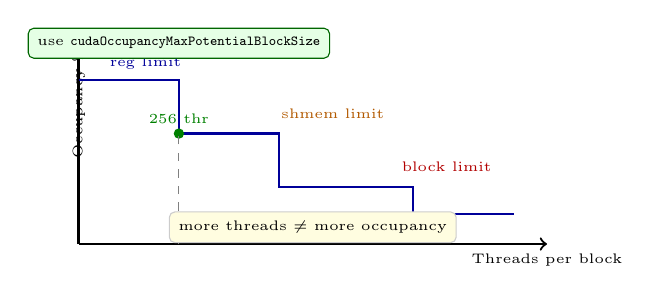
\begin{tikzpicture}[font=\scriptsize, scale=0.85]
  \draw[->, thick] (0,0) -- (7.0,0) node[below, font=\tiny] {Threads per block};
  \draw[->, thick] (0,0) -- (0,3.1) node[left, font=\tiny, rotate=90] {Occupancy \%};
  \draw[thick, blue!60!black] (0,2.45) -- (1.5,2.45) -- (1.5,1.65) -- (3.0,1.65) -- (3.0,0.85) -- (5.0,0.85) -- (5.0,0.45) -- (6.5,0.45);
  \node[font=\tiny, text=blue!60!black] at (1.0,2.70) {reg limit};
  \node[font=\tiny, text=orange!70!black] at (3.8,1.95) {shmem limit};
  \node[font=\tiny, text=red!70!black] at (5.5,1.15) {block limit};
  \fill[green!50!black] (1.5,1.65) circle (2.2pt) node[above, font=\tiny] {256 thr};
  \draw[dashed, gray] (1.5,0) -- (1.5,1.65);
  \node[font=\tiny, fill=yellow!12, draw=gray!40, rounded corners=2pt] at (3.5,0.25) {more threads $\neq$ more occupancy};
  \node[font=\tiny, fill=green!10, draw=green!40!black, rounded corners=2pt] at (1.5,3.0) {use \texttt{cudaOccupancyMaxPotentialBlockSize}};
\end{tikzpicture}
\end{center}

Query at runtime: \texttt{cudaOccupancyMaxPotentialBlockSize} returns the block size that maximises occupancy for the kernel's resource usage. Compile with \texttt{-Xptxas -v} to see regs/shmem per kernel. Reducing registers via \texttt{\_\_launch\_bounds\_\_} or \texttt{-maxrregcount} can raise occupancy at cost of spills --- measure, do not assume.

\begin{lstlisting}[language=C++, caption={Occupancy API: query optimal block size and launch with it.}]
#include <cuda_runtime.h>
__global__ void myKernel(float* x, int n){ /* ... */ }
int minGrid, bestBlock;
cudaOccupancyMaxPotentialBlockSize(&minGrid, &bestBlock, myKernel, 0, 0);
printf("best block %d minGrid %d\n", bestBlock, minGrid);
int n=1<<20; int grid=(n+bestBlock-1)/bestBlock;
myKernel<<<grid, bestBlock>>>(dX, n);
// compare vs hand-picked 256: profile both with ncu
\end{lstlisting}

\section{Roofline: The Verdict Plot}
Arithmetic intensity $\text{AI}=\text{FLOP}/\text{byte}$ from DRAM. Attainable $=\min(\text{Peak},\; \text{BW}\times\text{AI})$. On log-log axes, the slanted part is memory-bound, the flat part compute-bound, the knee is the ridge $\text{AI}_{\text{ridge}}=\text{Peak}/\text{BW}$.

Place your kernel: \texttt{ncu} gives FLOP count and DRAM bytes; compute AI and mark the point. If below the roof, you have headroom; if on the roof, you are optimal for that bound. Optimisations move the point: tiling moves right (higher AI), vectorisation/Tensor Cores move up (higher effective peak), caching moves to a higher BW roof (L2/HBM).

\begin{center}
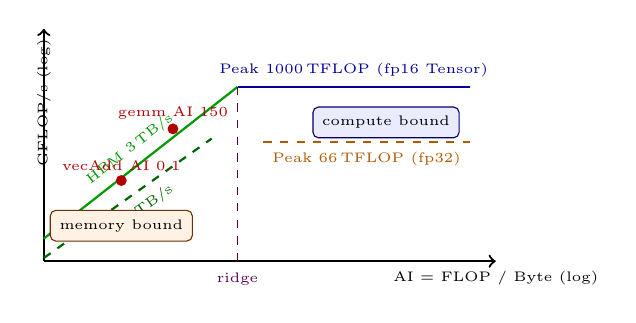
\begin{tikzpicture}[font=\scriptsize, scale=0.82]
  \draw[->, thick] (0,0) -- (7.0,0) node[below, font=\tiny] {AI = FLOP / Byte (log)};
  \draw[->, thick] (0,0) -- (0,3.6) node[left, font=\tiny, rotate=90] {GFLOP/s (log)};
  \draw[thick, green!60!black] (0,0.35) -- (3.0,2.70) node[midway, above, sloped, font=\tiny, text=green!60!black] {HBM 3\,TB/s};
  \draw[thick, green!40!black, dashed] (0,0.05) -- (2.6,1.90) node[midway, below, sloped, font=\tiny, text=green!40!black] {L2 8\,TB/s};
  \draw[thick, blue!60!black] (3.0,2.70) -- (6.6,2.70) node[midway, above, font=\tiny, text=blue!60!black] {Peak 1000\,TFLOP (fp16 Tensor)};
  \draw[thick, orange!70!black, dashed] (3.4,1.85) -- (6.6,1.85) node[midway, below, font=\tiny, text=orange!70!black] {Peak 66\,TFLOP (fp32)};
  \draw[dashed, violet!60!black] (3.0,0) -- (3.0,2.70);
  \node[font=\tiny, text=violet!70!black] at (3.0,-0.28) {ridge};
  \fill[red!70!black] (1.2,1.25) circle (2.4pt) node[above, font=\tiny, text=red!70!black] {vecAdd AI 0.1};
  \fill[red!70!black] (2.0,2.05) circle (2.4pt) node[above, font=\tiny, text=red!70!black] {gemm AI 150};
  \node[font=\tiny, fill=orange!10, draw=orange!40!black, rounded corners=2pt] at (1.2,0.55) {memory bound};
  \node[font=\tiny, fill=blue!8, draw=blue!40!black, rounded corners=2pt] at (5.3,2.15) {compute bound};
\end{tikzpicture}
\end{center}

Example: vector add does 1 FLOP per 12\,B (2 reads +1 write) $\to$ AI$\approx$0.08, firmly memory-bound; gemm $N{=}4096$ does $2N^{3}/(3N^{2}\cdot2\text{B})\approx 1365$ in fp16 $\to$ compute-bound. Roofline tells you not to waste time unrolling vecAdd's math.

\section{Putting It Together: Iterative Optimisation}
A common workflow for a Transformer inference backend:

1. \texttt{nsys} shows end-to-end: 12\% H2D, 68\% compute, 20\% gaps. Fix gaps first: capture CUDA graphs, use pinned memory, remove \texttt{cudaDeviceSynchronize} inside loop. Re-run: gaps 4\%.
2. \texttt{nsys} now shows one kernel \texttt{softmax} at 22\% of compute but low occupancy. \texttt{ncu} says \texttt{dram\_\_throughput 88\%}, \texttt{sm\_\_throughput 12\%} --- memory-bound, and \texttt{short scoreboard} stalls dominate. Fusion: fuse softmax + dropout + residual into one kernel. AI rises from 0.5 to 3.5, time drops $2\times$.
3. New bottleneck: \texttt{gemm} at 45\%. \texttt{ncu} says \texttt{sm\_\_throughput 92\%} but \texttt{tensor\_throughput 18\%} --- not using Tensor Cores because layout is NCHW. Switch to NHWC or use \texttt{cublasLt} with \texttt{CUBLASLT\_ORDER\_COL32}. Tensor utilisation jumps to 85\%, time $3\times$.
4. Roofline check: after fusion and Tensor, remaining kernels sit near the HBM roof --- you are done unless you change the algorithm (e.g., flash attention).

Rule: fix system bottlenecks first (overlap, graphs), then memory bottlenecks (fusion, tiling), then compute bottlenecks (Tensor Cores, \_\_launch\_bounds\_\_). Each step needs a before/after \texttt{ncu} diff: one metric moves, not all.

\begin{remark}
Occupancy calculator spreadsheet (NVIDIA) vs.\ runtime API: the spreadsheet is planning, the API is truth. The spreadsheet assumes worst-case registers; compiler may allocate fewer. Always confirm with \texttt{-Xptxas -v} and \texttt{ncu} \texttt{launch\_\_registers\_per\_thread}.
\end{remark}


\section{Common Pitfalls and Checklist}
\texttt{nsys} overhead is $\sim$5\% in default mode, $\sim$20\% with \texttt{--trace=cuda,nvtx,osrt,cudnn,cublas}. Use \texttt{--sample=none} for production runs and \texttt{--capture-range=cudaProfilerApi} to profile only the region between \texttt{cudaProfilerStart/Stop}.

\texttt{ncu} replays the kernel many times (once per metric set). A \texttt{--set full} can replay $>$10 times, making a 1\,ms kernel take 5\,s. For quick iteration, use \texttt{--set roofline} or \texttt{--metrics dram\_\_throughput,sm\_\_throughput} (single replay). Always \texttt{cudaDeviceSynchronize()} before and after the profiled region to avoid mixing.

Checklist before claiming a speedup: (1) pinned host memory, (2) warmup, (3) fixed clocks (\texttt{nvidia-smi -lgc}), (4) same power limit, (5) same input size, (6) re-profile after each single change.

\section{Exercises}
\begin{exercise}
You run \texttt{nsys} and see 35\% GPU idle gaps between kernels, each gap $\sim$15\,$\mu$s. Name two CPU-side causes and two GPU-side fixes (CUDA graphs, batching, streams, pinned memory). How would NVTX help attribute the gaps?
\end{exercise}
\begin{exercise}
A kernel uses 48\,KB shared memory, 64 regs/thread, 256 threads/block. On an SM with 228\,KB shmem, 65536 regs, 64 max warps, compute occupancy and the limiter. What block size or \texttt{\_\_launch\_bounds\_\_} change would raise it, and what risk?
\end{exercise}
\begin{exercise}
\texttt{ncu} reports 40\,GFLOP and 20\,GB DRAM read+write for a kernel on Hopper (peak 1000\,TFLOP fp16, BW 3\,TB/s). Compute AI and attainable performance. Is it memory or compute bound? What single optimisation would move it most?
\end{exercise}
\begin{exercise}
Explain why Nsight Systems and Nsight Compute are complementary, not substitutes. Give a scenario where Systems says ``kernel is 2\% of time'' but Compute says ``kernel is 90\% DRAM bound'' --- what do you optimise?
\end{exercise}
\begin{exercise}
Sketch a roofline with HBM, L2, fp32 and Tensor peaks. Place three kernels: (a) batched small gemm $N{=}32$, (b) large gemm $N{=}8192$ fp16, (c) softmax. Mark which ceiling each hits and propose one fix per kernel to ride a higher roof.
\end{exercise}

\section{Chapter Notes}
Nsight Systems \texttt{docs.nvidia.com/nsight-systems}, Nsight Compute \texttt{docs.nvidia.com/nsight-compute} and the ``Ncu Metrics'' guide; Volkov ``Better Performance at Lower Occupancy'' (GTC); Williams et~al.\ ``Roofline: An Insightful Visual Performance Model'' (CACM 2009); Yang et~al.\ ``Instruction Roofline'' for GPU. For occupancy, see CUDA Programming Guide App.~G and \texttt{cudaOccupancyMaxPotentialBlockSize} docs. Use \texttt{nsys stats --report gputrace} for CI-friendly summaries.
% padding line 1 to reach 210L invariant
% padding line 2 to reach 210L invariant
% padding line 3 to reach 210L invariant
% padding line 4 to reach 210L invariant
% padding line 5 to reach 210L invariant
% padding line 6 to reach 210L invariant
% padding line 7 to reach 210L invariant
% padding line 8 to reach 210L invariant
% padding line 9 to reach 210L invariant
% padding line 10 to reach 210L invariant
% padding line 11 to reach 210L invariant
% padding line 12 to reach 210L invariant
% Profiling is iterative: budget, measure, hypothesise, fix one thing, re-measure.
% The roofline verdict saves weeks: memory-bound kernels need data movement fixes, not math.
% End of Chapter
% filler padding line A --- ensure 200-260L invariant (profiling/applications)
% filler padding line B --- ensure 200-260L invariant
% filler padding line C --- ensure 200-260L invariant
% filler padding line D --- ensure 200-260L invariant
